\documentclass [12pt,oneside] {article}

% Codificação dos caracteres da entrada (use ISO no Windows e UTF no Linux)
%\usepackage[isolatin]{inputenc}  % arquivos LaTeX em ISO-8859-1
\usepackage[utf8]{inputenc}     % arquivos LaTeX em Unicode

% packages usados na construção deste documento
\usepackage [T1]{fontenc}        % caracteres acentuados corretos na saida
\usepackage {times}              % Fontes Times
\usepackage [portuguese]{babel}      % texto em portugues
\usepackage {indentfirst}        % indentar primeiro paragrafo
\usepackage {epsfig}             % inclusao de figuras em formato EPS
\usepackage[hidelinks]{hyperref}
\usepackage{float}				 % para imagens

% usar papel no formato A4 com margens 30,30,25,25 mm^M
\usepackage[a4paper,top=30mm,bottom=30mm,left=25mm,right=25mm]{geometry}

% relaxar o espaçamento entre caracteres
% \sloppy

% O espaçamento entre linhas deve ser 1.5
% \renewcommand{\baselinestretch}{1.5}

% indentação dos parágrafos é 15mm
\setlength{\parindent}{15mm}

% pacote sugerido para formata��o de c�digo-fonte
\usepackage{listings}
\lstset{language=c}
\lstset{inputencoding=latin1,extendedchars=true}
\lstset{basicstyle=\small,commentstyle=\textit,stringstyle=\ttfamily}
\lstset{showspaces=false,showtabs=false,showstringspaces=false}
\lstset{numbers=left,stepnumber=5,numberstyle=\tiny}
\lstset{columns=flexible,mathescape=true}
\lstset{frame=single}

% pacote sugerido para formatação de algoritmos
\usepackage{algorithm,algorithmic}
\floatname{algorithm}{Algoritmo}
\renewcommand{\algorithmiccomment}[1]{~~~// #1}
 % incluir pacotes e configurações

%=====================================================

\begin {document}

\title {Modelo e Exemplo de Relatório em \LaTeX}
\author {Carlos Maziero}
\date {Agosto de 2007}
\maketitle

%=====================================================

\section{Introdução}

Este é um modelo e exemplo de relatório preparado em \LaTeX. Para obter os melhores resultados, compile este modelo usando a seguinte sequência de passos:

\begin{footnotesize}
\begin{verbatim}
> latex  main                 // compilação inicial
> bibtex main                 // gera referências
> latex  main                 // compilação final
> dvips -tA4 -Ppdf main.dvi   // gera o PostScript
> ps2pdf main.ps              // converte PostScript em PDF
\end{verbatim}
\end{footnotesize}

Um arquivo \texttt{Makefile} foi preparado Para facilitar a compilação deste documento. Para conhecer seu funcionamento, basta digitar \texttt{make} no diretório principal deste modelo.

Um bom guia introdutório de \LaTeX\ disponível na Internet é \cite{oetiker07}, que também tem uma versão em português. Para tópicos mais avançados consulte \cite{goossens93}.

%=====================================================

\section{Estrutura do texto}

Para melhorar a legibilidade do texto, deve ser extremamente evitado o uso de sub-divisões mais profundas que a sub-seção (por exemplo, sub-sub-seções). Se elas forem absolutamente necessárias, não devem ser numeradas. Deve-se analisar a possibilidade de uso de uma lista de itens em seu lugar. O número de níveis de texto do documento não deve exceder dois: seção e sub-seção. O uso de mais que dois níveis dificulta a leitura e prejudica muito a estética do texto.

%=====================================================

\section{Exemplo de figura}

A forma sugerida para incluir figuras em um documento \LaTeX\ é importá-las no formato EPS (\emph{Extended PostScript}), usando o pacote \texttt{epsfig}. A maior parte das ferramentas permite exportar figuras em formato EPS (a figura do exemplo foi produzida com o \emph{Inkscape}, um programa livre para Windows e Linux). A figura \ref{comun-intra-inter} mostra um exemplo de inclusão de figura nesse formato. Para mais informações consulte \cite{goossens93}.

% exemplo de inserção de figura
\begin{figure}[!htb]
\centering
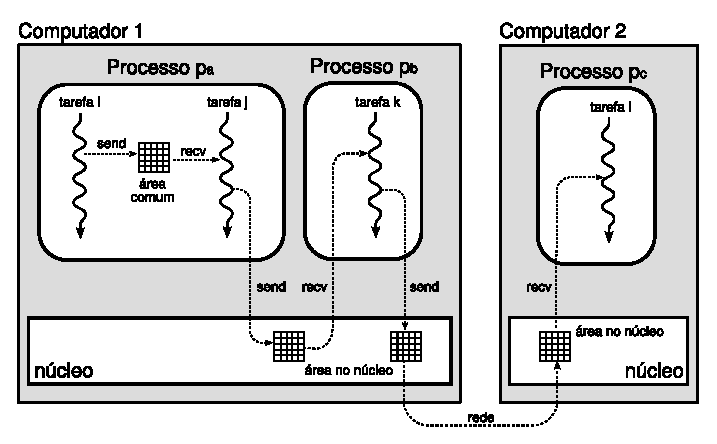
\includegraphics[width=12cm]{exemplo.eps}
\caption{Comunicação inter-processos.}
\label{comun-intra-inter}
\end{figure}

%=====================================================

\section{Exemplo de tabela}

Tabelas são elementos importantes de um documento. No \LaTeX\ as tabelas podem ser objetos flutuantes (definidas no ambiente \texttt{table} e referenciadas por números usando \texttt{label} e \texttt{ref}) ou objetos fixos simples, criados pelo ambiente \texttt{tabular}. A tabela \ref{modelos} é um exemplo de tabela flutuante, cuja posição no texto pode variar em função das quebras de página.

\begin{table}[!htp]
\centering
\caption{Os 16 modelos centrais do UCON$_{\mathrm{ABC}}$}
\label{modelos}
\begin{tabular}{|c|cccc|}
\cline{2-5}
\multicolumn{1}{c|}{}& 0 (imutável) & 1 (\emph{pre-update}) & 2 (\emph{on-update}) & 3 (\emph{pos-update}) \\
\hline
\texttt{preA} & \textbullet & \textbullet & -- & \textbullet \\
\hline
\texttt{onA} & \textbullet & \textbullet & \textbullet & \textbullet \\
\hline
\texttt{preB} & \textbullet & \textbullet & -- & \textbullet \\
\hline
\texttt{onB} & \textbullet & \textbullet & \textbullet & \textbullet \\
\hline
\texttt{preC} & \textbullet & -- & -- & -- \\
\hline
\texttt{onC} & \textbullet & -- & -- & -- \\
\hline
\end{tabular}
\end{table}

%=====================================================

\section{Exemplo de equação}

Equações podem estar dentro do texto, como esta: $E=m\times c^2$, ou destacadas e numeradas como segue:

\begin{equation}
E = m \times c^2
\end{equation}

%=====================================================

\section{Exemplos de código-fonte}

Códigos-fonte podem ser produzidos de forma simples através do ambiente \texttt{verbatim}, como mostra este exemplo:

\begin{footnotesize}
\begin{verbatim}
#include <stdio.h>

int main (int argc, char *argv[])
{
   int i ;                           // uma variável local

   for (i=0; i< 100; i++)            // um laço for
      printf ("i vale %d\n", i) ;    // uma saída na tela
}
\end{verbatim}
\end{footnotesize}

No entanto, é preferível usar pacotes especializados para a edição ou inclusão de códigos-fonte, como o pacote \texttt{listings}. Eis um exemplo de código-fonte escrito com esse pacote:

% exemplo de código-fonte definido no próprio texto
\begin{lstlisting}
#include <stdio.h>

int main (int argc, char *argv[])
{
   int i ;                           // uma variável local

   for (i=0; i< 100; i++)            // um laço for
      printf ("i vale %d\n", i) ;    // uma saída na tela
}
\end{lstlisting}

Esse pacote também permite incluir códigos-fonte de arquivos externos:

% exemplo de código-fonte incluso
\lstinputlisting{exemplo.c}

%=====================================================

\section{Exemplo de algoritmo}

Os pacotes \texttt{algorithm} e \texttt{algorithmic} permitem formatar algoritmos facilmente:

\begin{algorithm}[H]
\caption{Ações de $s_i$ ao encerrar um ciclo:}
\label{on-period-ending}
\begin{small}
\begin{algorithmic}[1]
\FORALL{$x \in \mathcal{K}_i$}
  \STATE{$\mathit{banned}_i(x) \gets$ FALSE}
  \STATE{$mi_i(x) \gets 0$}
  \STATE{$mm_i(x) \gets 0$}
  \STATE{$\mathit{age}_i(x) \gets \mathit{age}_i(x) + 1$}
  \IF{$\mathit{age}_i(x) = \mathit{age}_\mathit{max}$}
     \STATE{$\mathcal{K}_i \gets \mathcal{K}_i - \{x\}$}
     \COMMENT{``esquece'' do servidor $x$}
     \STATE{remove as informações locais sobre $x$}
     \STATE{envia $\mathit{notify}(x,\mathit{undef})$ ao grupo de confiança $\mathcal{T}_i$}
  \ENDIF
\ENDFOR
\end{algorithmic}
\end{small}
\end{algorithm}
 
%=====================================================

\section{Conclusão}

Todo relatório deve encerrar com uma pequena conclusão, resumindo os tópicos apresentados e os eventuais resultados obtidos pelo autor, quando for o caso.

%=====================================================

% definição do estilo e inclusão da bibliografia
\bibliographystyle{plain}
\bibliography{referencias}

\end{document}

%=====================================================
